\documentclass{beamer}

\setlength{\parskip}{\baselineskip}
\setlength{\parindent}{0pt}
\usepackage{default}
\usepackage{tabularx}
\usepackage{url}
\usepackage{graphicx}

\title{\huge{Why PGFPlots is better than Matlab's figures?}}
\author{Manuel Baumann}
\titlegraphic{
   \vspace{-1cm}
   \includegraphics[scale=0.08]{images/TU_Delft_logo1.png}\hspace{4cm}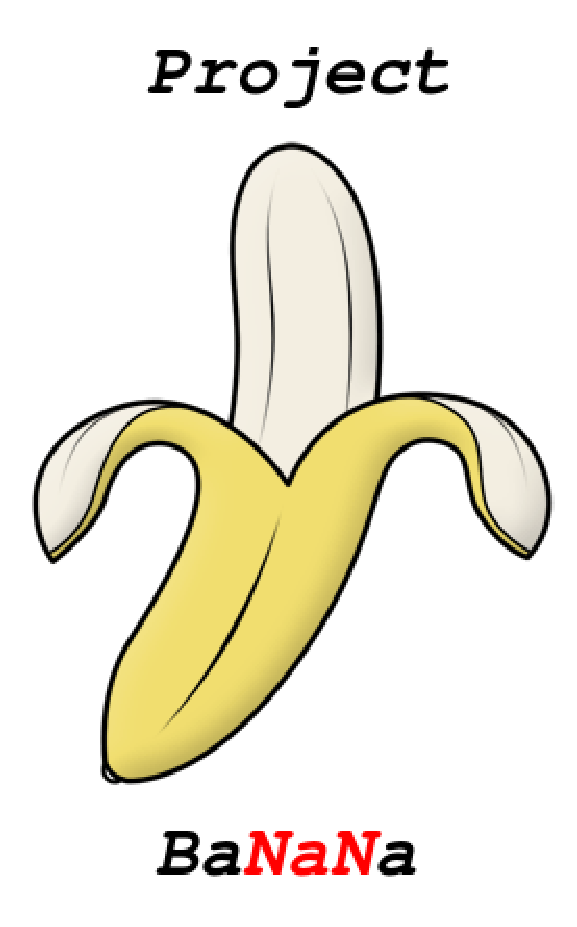
\includegraphics[scale=0.15]{../../images/logo}}
\date{\footnotesize{September 24, 2015}}
\begin{document}

\frame{\titlepage}
\begin{frame}
\frametitle{What is PGFPlots ?}
A plot in a high-end \LaTeX \ document should:
\begin{itemize}
 \item be font-consistent,
 \item 
\end{itemize}
\end{frame}

\begin{frame}
\frametitle{Example: The young Manuel...}
\begin{figure}
 \includegraphics[width=0.8\textwidth]{images/matlab.png}
\end{figure}
\end{frame}

\begin{frame}
\frametitle{Example: How is looks in SISC}
\begin{figure}
 \includegraphics[width=0.8\textwidth]{images/matlab_bw.png}
\end{figure}
\end{frame}

\begin{frame}
\frametitle{Example: How is REALLY looks in SISC}
\begin{figure}
 \includegraphics[width=0.4\textwidth]{images/matlab_bw.png} \hspace{0.6cm} \includegraphics[width=0.4\textwidth]{images/matlab_bw.png} 
\end{figure}
\end{frame}

\begin{frame}
\frametitle{We need to talk...}
Ideas for the new academic year
\begin{itemize}
 \item new webmaster
 \item baNaNa talks
 \item $SIAM \ CFD^2ay \ 2016$
 \item chess competition 
\end{itemize}
\end{frame}

\begin{frame}
\frametitle{Further reading}
Many information are available online:
\begin{itemize}
 \item \url{https://github.com/}
 \item \url{http://try.github.io/levels/1/challenges/1}
 \item \url{http://git-scm.com/book}
\end{itemize}
These slides, and much more, will be published at:
\begin{itemize}
 \item \url{http://projectbanana.github.io/}
\end{itemize}
 \begin{figure}
\centering
 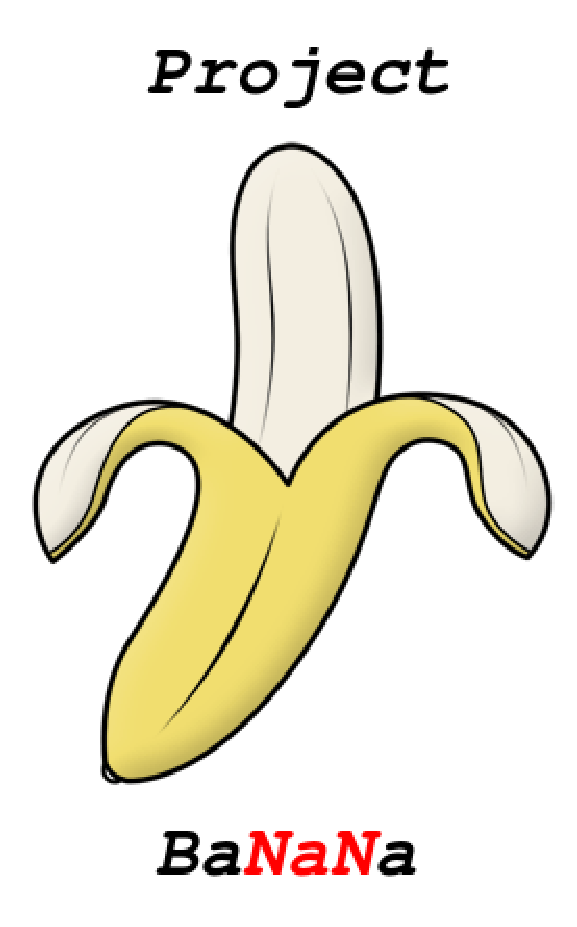
\includegraphics[height=0.3\textheight]{../../images/logo}
\end{figure}
\end{frame}

\end{document}
